\documentclass[a4paper,12pt]{article}
\usepackage[a4paper, top=2cm,bottom=2cm,right=2cm,left=2cm]{geometry}

\usepackage{bm,xcolor,mathdots,latexsym,amsfonts,amsthm,amsmath,
					mathrsfs,graphicx,cancel,tikz-cd,hyperref,booktabs,caption,amssymb,amssymb,wasysym}
\hypersetup{colorlinks=true,linkcolor=blue}
\usepackage[italian]{babel}
\usepackage[T1]{fontenc}
\usepackage[utf8]{inputenc}
\newcommand{\s}[1]{\left\{ #1 \right\}}
\newcommand{\sbarra}{\backslash} %% \ 
\newcommand{\ds}{\displaystyle} 
\newcommand{\alla}{^}  
\newcommand{\implica}{\Rightarrow}
\newcommand{\iimplica}{\Leftarrow}
\newcommand{\ses}{\Leftrightarrow} %se e solo se
\newcommand{\tc}{\quad \text{ t. c .} \quad } % tale che 
\newcommand{\spazio}{\vspace{0.5 cm}}
\newcommand{\bbianco}{\textcolor{white}{,}}
\newcommand{\bianco}{\textcolor{white}{,} \\}% per andare a capo dopo 																					definizioni teoremi ...


% campi 
\newcommand{\N}{\mathbb{N}} 
\newcommand{\R}{\mathbb{R}}
\newcommand{\Q}{\mathbb{Q}}
\newcommand{\Z}{\mathbb{Z}}
\newcommand{\K}{\mathbb{K}} 
\newcommand{\C}{\mathbb{C}}
\newcommand{\F}{\mathbb{F}}
\newcommand{\p}{\mathbb{P}}

%GEOMETRIA
\newcommand{\B}{\mathfrak{B}} %Base B
\newcommand{\D}{\mathfrak{D}}%Base D
\newcommand{\RR}{\mathfrak{R}}%Base R 
\newcommand{\Can}{\mathfrak{C}}%Base canonica
\newcommand{\Rif}{\mathfrak{R}}%Riferimento affine
\newcommand{\AB}{M_\D ^\B }% matrice applicazione rispetto alla base B e D 
\newcommand{\vett}{\overrightarrow}
\newcommand{\sd}{\sim_{SD}}%relazione sx dx
\newcommand{\nvett}{v_1, \, \dots , \, v_n} % v1 ... vn
\newcommand{\ncomb}{a_1 v_1 + \dots + a_n v_n} %a1 v1 + ... +an vn
\newcommand{\nrif}{P_1, \cdots , P_n} 
\newcommand{\bidu}{\left( V^\star \right)^\star}

\newcommand{\udis}{\amalg}
\newcommand{\ric}{\mathfrak{U}}
\newcommand{\inclu}{\hookrightarrow }
%ALGEBRA

\newcommand{\semidir}{\rtimes}%semidiretto
\newcommand{\W}{\Omega}
\newcommand{\norma}{\vert \vert }
\newcommand{\bignormal}{\left\vert \left\vert}
\newcommand{\bignormar}{\right\vert \right\vert}
\newcommand{\normale}{\triangleleft}
\newcommand{\nnorma}{\vert \vert \, \cdot \, \vert \vert}
\newcommand{\dt}{\, \mathrm{d}t}
\newcommand{\dz}{\, \mathrm{d}z}
\newcommand{\dx}{\, \mathrm{d}x}
\newcommand{\dy}{\, \mathrm{d}y}
\newcommand{\amma}{\gamma}
\newcommand{\inv}[1]{#1^{-1}}
\newcommand{\az}{\centerdot}
\newcommand{\ammasol}[1]{\tilde{\gamma}_{\tilde{#1}}}
\newcommand{\pror}[1]{\mathbb{P}^#1 (\R)}
\newcommand{\proc}[1]{\mathbb{P}^#1(\C)}
\newcommand{\sol}[2]{\widetilde{#1}_{\widetilde{#2}}}
\newcommand{\bsol}[3]{\left(\widetilde{#1}\right)_{\widetilde{#2}_{#3}}}
\newcommand{\norm}[1]{\left\vert\left\vert #1 \right\vert \right\vert}
\newcommand{\abs}[1]{\left\vert #1 \right\vert }
\newcommand{\ris}[2]{#1_{\vert #2}}
\newcommand{\vp}{\varphi}
\newcommand{\vt}{\vartheta}
\newcommand{\wt}[1]{\widetilde{#1}}
\newcommand{\pr}[2]{\frac{\partial \, #1}{\partial\, #2}}%derivata parziale
%per creare teoremi, dimostrazioni ... 
\theoremstyle{plain}
\newtheorem{thm}{Teorema}[section] 
\newtheorem{ese}[thm]{Esempio} 
\newtheorem{ex}[thm]{Esercizio} 
\newtheorem{fatti}[thm]{Fatti}
\newtheorem{fatto}[thm]{Fatto}

\newtheorem{cor}[thm]{Corollario} 
\newtheorem{lem}[thm]{Lemma} 
\newtheorem{al}[thm]{Algoritmo}
\newtheorem{prop}[thm]{Proposizione} 
\theoremstyle{definition} 
\newtheorem{defn}{Definizione}[section] 
\newcommand{\intt}[2]{int_{#1}^{#2}}
\theoremstyle{remark} 
\newtheorem{oss}{Osservazione} 
\newcommand{\di }{\, \mathrm{d}}
\newcommand{\tonde}[1]{\left( #1 \right)}
\newcommand{\quadre}[1]{\left[ #1 \right]}
\newcommand{\w}{\omega}

% diagrammi commutativi tikzcd
% per leggere la documentazione texdoc

\begin{document}
\textbf{Lezione del 29 aprile}
\begin{ese}Calcolare 
$$\int_0^{+\infty} \frac{1}{1+x^n}\dx$$ 
Scegliamo come regione 
$$ D_R =\s{ z\in \C \, : \, \abs{z} < R \text{  e } 0<arg(z) < \frac{2\pi}{n}}$$ 
$z_0=e^{i\frac{\pi}{n}}$ \`e l'unico polo di $f(z) = \frac{1}{1+z^n}$ in $D_R$.\\
Osserviamo che 
$$Res(f,z_0) = \frac{1}{nz_0^{n-1}} =\frac{z_0}{nz_0^n} =-\frac{z_0}{n} = \frac{1}{n} \tonde{-\cos \frac{\pi}{n}-i\sin \frac{\pi}{n}}$$
Consideriamo le seguenti parametrizzazioni
$$ \alpha_R(t)  =t \text{ per } t\in [0, R]$$
$$ \beta_R(t)  =Re^{it} \text{ per } t\in \quadre{0, \frac{2\pi}{n}}$$
$$ \gamma_R(t)  =te^{\frac{2\pi}{n}} \text{ per } t\in [0, R]$$
\begin{figure}[!h]
\centering
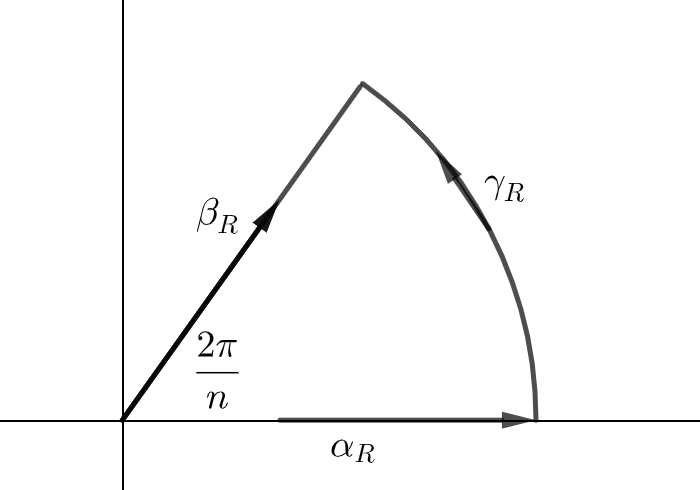
\includegraphics[scale=0.5]{Figure/04_29}
\end{figure}
Allora per il teorema dei residui si ha 
$$ \int_{\alpha_R} f(z) \dz + \int_{\gamma_R} f(z) \dz - \int_{\beta_R} f(z) \dz = \frac{2\pi i}{n}\tonde{-\cos \frac{\pi}{n}-i\sin\frac{\pi}{n} } =\frac{2\pi}{n}\tonde{\sin \frac{\pi}{n}-i\cos\frac{\pi}{n}} $$
Osserviamo che $\int_{\alpha_R} f(z) \dz$ \`e quello che vogliamo effettivamente calcolare.\\
Andiamo a vedere cosa succede lungo $\gamma_R$
\begin{equation}
\label{fattogenerale}
\begin{split}
\abs{\int_{\gamma_R} f(z) \dz }=\abs{\int_0^{\frac{2\pi}{n}} f(\gamma_R(r)) \gamma'_R(t) \dt }  \leq \int_0^{\frac{2\pi}{n}} \abs{\frac{1}{1+\tonde{Re^{it}}^n} iRe^{it}} \dt \leq\\
\leq  \int_0^{\frac{2\pi}{n}} \frac{R}{R^n-1} \dt =\frac{2\pi R}{n(R^n-1)} \to 0 \text{ per } R\to \infty
\end{split}
\end{equation}
Resta da osservare cosa succede lungo $\beta_R$
$$ \int_{\beta_R} f(z) \dz = \int_0^R f\tonde{\beta_R(t)} \beta'_R(t) \dt = \int_0^R \frac{1}{\tonde{ 1 + Re^{\frac{2\pi}{n}i}}^n} e^{\frac{2\pi }{n}i} \dt  =\int_0^R \frac{1}{1+t^n} e^{\frac{2\pi }{n}i}\dt  =$$
$$=e^{\frac{2\pi}{n}i} \int_0^R \frac{\dt }{1+t^2}=e^{\frac{2\pi}{n}i} \int_{\alpha_R} f(z) dz $$ 
dunque passando al limite per $R \to \infty$ e ponendo $I= \int_0^\infty \frac{1}{1+t^n}\dt $ da 
$$ \int_{\alpha_R} f(z) \dz + \int_{\beta_R} f(z) \dz -\int_{\gamma_R} f(z) \dz = \frac{2\pi}{n}\tonde{\sin \frac{\pi}{n}-i\cos\frac{\pi}{n}}$$
otteniamo 
$$ I + 0 + e^{\frac{2\pi}{n} i } I =  \frac{2\pi}{n}\tonde{\sin \frac{\pi}{n}-i\cos\frac{\pi}{n}}$$
Poich\`e $I\in \R$ otteniamo, uguagliando la parte immaginaria 
$$ I \sin \frac{\pi}{n} = \frac{2\pi}{n}\cos\frac{\pi}{n} \quad \implica \quad I 2\sin \frac{\pi}{n}\cos \frac{\pi}{n} =2\frac{\pi}{n}\cos \frac{\pi}{n}$$ 
dunque 
$$ \int_0^\infty \frac{1}{1+t^2}\dt =\frac{\pi}{n}\cdot\frac{1}{\sin\frac{\pi}{n}}$$
\end{ese}
\spazio

\begin{oss}Possiamo generalizzare quanto visto in \ref{fattogenerale} come segue:\\
Se $\ds \lim_{R\to +\infty} RM(R) = 0$ allora $$\lim_{R\to +\infty} \int_{\gamma_R} f(z)\dz =0$$
dove $\gamma_R$ parametrizza una porzione di  circonferenza di raggio $R$, centrata nell'origine e con parte immaginaria non negativa
\end{oss}
\spazio
Prima del prossimo esempio occorrono $2$ lemmi 
\begin{lem}Sia $f$ meromorfa con polo semplice in $0$ e sia 
$$ \gamma_\varepsilon:\, [0, 2\pi] \to \C\setminus\s 0 \quad \gamma_\varepsilon(t) = \varepsilon e^{it} \text{ per } \varepsilon>0$$
Allora 
$$ \lim_{\varepsilon\to 0 } \int_{\gamma_\varepsilon} f(z) \dz = \pi i Res(f,0)$$
\proof Si ha $f(z) = \frac{a_{-1}}{z} +g(z)$ dove $g$ \`e olomorfa in un intorno di $0$ con primitiva $G$
$$ \int_{\gamma_\varepsilon} f(z) \dz = \int_{\gamma_\varepsilon} \frac{a_{-1}}{z}\dz + \int_{\gamma_\varepsilon} g(z) \dz = \pi i a_{-1} + G\tonde{\delta_\varepsilon(\pi)} - G\tonde{\delta_\varepsilon(0)}$$ 
dunque per $\varepsilon\to 0$ otteniamo la tesi
\end{lem}
\spazio
Per le stime sulle semicirconferenze ``grandi" usiamo 
\begin{lem}$f$ meromorfa su $\C$ tale che $\ds \lim_{R\to \infty} M(R)=0$ allora 
$$ \lim_{R\to \infty }\int_{\gamma_R} f(z)  e^{iz}\dz =0$$
\proof Se $z=\gamma_R(t)=R \cos t + i R \sin t $ allora 
$$ e^{iz} =e^{iR\cos t } e^{-R\sin t } \quad \implica \quad \abs{e^{iz}} =e^{-R\sin t }$$ 
dunque 
$$ \abs{\int_{\gamma_R} f(z) e^{iz} \dz } \leq \int_0^\pi \abs{f\tonde{\gamma_R(t)} e^{i\gamma_R(t)} \gamma'_R(t)} \dt =\int_0^\pi \abs{f\tonde{\gamma_R(t)}} \cdot \abs{e^{i\gamma_R(t)}} \cdot \abs{ R i e^{it}} \leq \int_0^\pi M(r) e^{-R\sin t }  R \dt $$
$$ M(R) \int_0^\pi e^{-R\sin t } R \dt $$
Mostriamo che l'ultimo integrale \`e limitato indipendentemente da $R$ .\\
Ora su $\left[ 0, \frac{\pi}{2}\right]$ la funzione $\frac{\sin t }{t}$ \`e limitato dal basso da una costante $k$ (in tale intervallo \`e una funzione continua strettamente positiva su un compatto)\\
Allora 
$$ \int_0^\pi R e^{-R\sin t} \dt = 2\int_0^{\frac{\pi}{2}} Re^{-R\sin t } \dt = 2R \int_0^{\frac{\pi}{2}} e^{R \frac{\sin t}{t} t } \dt \leq 2 R \int_0^{\frac{\pi}{2}} e^{-Rkt} \dt = 2 \cancel{R} \left[ \frac{e^{-Rkt}}{\cancel{R}k} \right]_0^{\frac{\pi}{2}} = $$
$$ = \frac{2}{k}\tonde{-e^{Rk\frac{\pi}{2}}+1} \leq \frac{2}{k}$$

\begin{oss}Se non ci fosse il termine $e^{iz}$ la condizione che serviva era $\lim_{R \to  +\infty} R M(R)=0$, il fattore oscillante rende sufficiente una condizione pi\`u debole
\end{oss}
\end{lem}

\begin{ese}Calcoliamo 
$$ \int_0^\infty \frac{\sin x}{x}$$
dove estendiamo $\frac{\sin x }{x}$ in $0$ ponendolo uguale ad $1$.\\
Il fatto che l'integrale non converga assolutamente, ci induce a pensare che la stima sui termini che dovranno andare a $0$ sar\`a pi\`u file (non baster\`a pi\`u prendere i moduli).\\
Osserviamo che $$\int_0^\infty \frac{\sin x}{x} \dx =\lim_{R \to +\infty} \int_{\frac{1}{R}}^R \frac{\sin x }{x} \dx =\frac{1}{2}\tonde{\lim_{R\to \infty} \int_{-R}^{\frac{1}{R}}\frac{\sin x }{x} \dx + \int_{\frac{1}{R}}^R \frac{\sin x}{x} \dx } $$ dove abbiamo usato la parit\`a di $\frac{\sin x }{x}$.\\
Prendiamo come curva 
$$ \beta = \alpha_R \star \overline{\gamma_{\frac{1}{R}}} \star \beta_R \star \gamma_R$$ 
come in figura\\ 
\begin{figure}[!h]
\centering
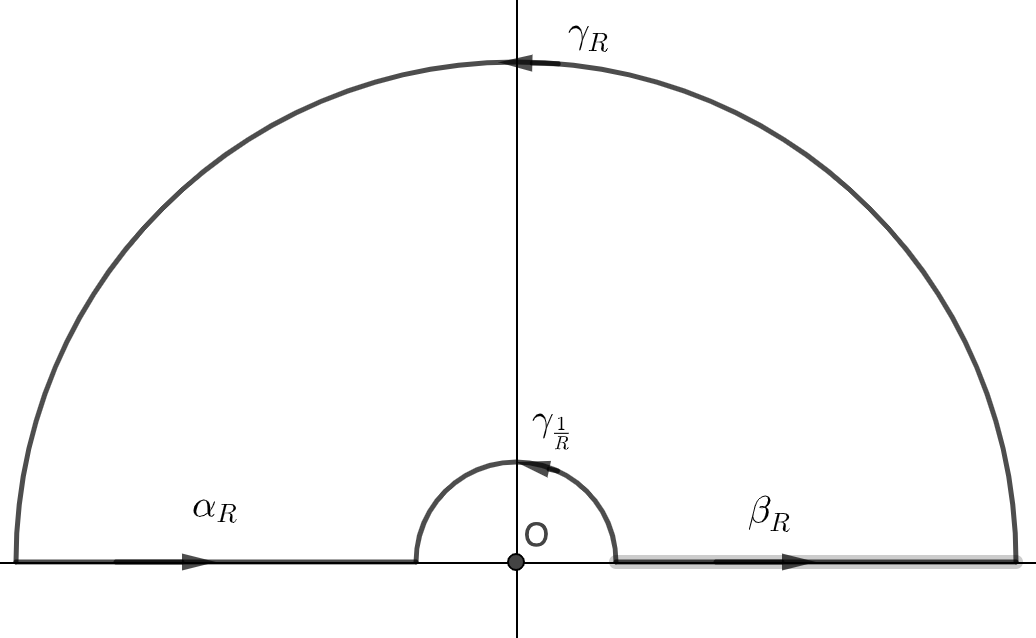
\includegraphics[scale=0.4]{Figure/04_29_1}
\end{figure}

Ora $\beta$ parametrizza il bordo di una regione (che \`e un disco topologico) che non contiene poli di $f$ dunque dal teorema dei residuo
$$ \int_{\alpha_R} f(z)\dz + \int_{\overline{\gamma_{\frac{1}{R}}}} f(z) \dz  + \int_{\beta_R} f(z) \dz + \int_{\gamma_R} f(z) \dz =0$$ 
Dal primo lemma si ha per $R \to \infty$
$$ \int_{\overline{\gamma_{\frac{1}{R}}}} f(z) \dz = -\pi i Res (f,0) =-\pi i $$
Mentre per il secondo lemma $\int_{\gamma_R} \to 0$ per $R \to + \infty$.\\
Ora passando al limite $R \to \infty$ e considerando solo le parti immaginarie otteniamo 
$$ 2\int_0^\infty\frac{\sin x}{x} \dx = \pi \quad \implica\quad \int_0^\infty\frac{\sin x}{x} \dx = \frac{\pi}{2}$$
\end{ese}
\newpage
\section{Derivata logaritmica}
Sia $f$ una funzione meromorfa su un aperto $\W \subseteq \C$ e sia $z_0$ un polo di $f$ per cui $f(z) = (z-z_0)^k g(z) $ con $g(z_0)\neq 0 $.\\
La derivata logaritmica di $f$  \`e $$\frac{f'}{f} $$
tale funzione \`e olomorfa eccetto al pi\`u nei poli o negli zeri di $f$.\\
Vediamo come si comporta ``vicino" a $z_0$
$$ f'(z) = k(z-z_0)^{k-1}g(z) + (z-z_0)^k g'(z)$$
per cui 
$$ \frac{f'(z)}{f(z)}=\frac{k}{z-z_0} +\frac{g'(z)}{g(z_0)}$$
Dunque la derivata logaritmica di $f$ ha un polo semplice in $z_0$ e il suo residuo in $z_0$ \`e $k$
\begin{oss}La derivata prende questo nome in quanto $d(\log(f))= \frac{f'}{f}$.\\
Inoltre se $k>0$ si ha $z_0$ uno zero, altrimenti un polo
\end{oss}
\begin{cor}Sia $f$ meromorfa su $\W$ e sia $R\subseteq \W$ una regione compatta con bordo $C^1$ a tratti.\\
Allora $R$ contiene un numero finito di zeri e poli di $f$ (sono discreti in un compatto) e supponiamo che nessuno di essi sia in $\partial R$.\\
Allora 
$$ \int_{\partial R} \frac{f'(z)}{f(z)}\dz =2\pi i (Z- P)$$
dove $Z$ indica il numero di zeri di $f$ e $P$ quello di poli (contati con molteplicit\`a)
\proof Segue dal teorema dei residui e dal conto fatto precedentemente  infatti se $k$ (quello di sopra) \`e positivo $z_0$ \`e uno zero con molteplicit\`a $k$ , se \`e negativo \`e un polo di ordine $-k$
\end{cor}
\begin{cor}[Teorema di Rouch\`e]\bianco
Sia $f:\, \W \to \C$ una funzione olomorfa e $R\subseteq \W$ una regione compatta con bordo $C^1$ a tratti.\\
Sia $g:\, \W \to \C$ olomorfa con $\abs{g(z)} < \abs{f(z)}$ per ogni $z\in \partial R$.\\
Allora $f$ e $f+g$ hanno lo steso numero di zeri (contati con molteplicit\`a) in $R$
\proof Da $\abs{g(z)} <\abs{f(z)}$ per ogni $z\in \partial R$ si deduce che $f$ \`e pi\`u in generale $h_t = f+tg$ non si annullino in $\partial R$  per ogni $t\in [0,1]$.\\
Inoltre $h_t$ \`e olomorfa essendo somma di funzioni olomorfe.\\
Applicando il corollario precedente a $h_t$ otteniamo che se $Z_t$ \`e il numero di zeri di $h_t$ allora 
$$ Z_t = \int_{\partial R} \frac{h_t'}{h_t}(z) \dz $$ 
Ora al variare di $t$ il membro di sinistra varia in maniera continua, dunque $Z_t$ \`e costante (funzione continua a valori interi) concludiamo osservando che $Z_0=Z_1$ dunque la tesi
\end{cor}
\begin{cor}[Teorema fondamentale dell'algebra]\bianco
Sia $p(z) = z^n + a_{n-1} z^{n-1} +\dots + a_0$, se $M= \max\s{\abs{a_i}}$ allora $p$ ammette $n$ radici (contate con molteplicit\`a) nel disco di raggio $M+1$ centrato nell'origine.
\proof Sia 
$$g(z) = p(z) - z^n = \sum_{i=0}^{n-1} a_i z^i$$ 
Allora se $\abs{z} > M+1$ si ha 
$$ \abs{g(z)} < \sum_{i=0}^{n-1} \abs{a_i z^i} \leq \sum_{i=0}^{n-1} M \abs{z}^i = M \frac{\abs{z}^n -1}{\abs z -1} \leq \abs z ^n -1 \leq \abs z^n$$
Per il teorema di Rouch\`e $f(z)= z^n$ e $p(z) = f(z) + g(z)$ hanno lo stesso numero di zeri in $B(0, R+1)$. Poich\`e $z^n$ ha $n$ zeri in  tale palla, segue la tesi 
\end{cor}
\end{document}